%%%%%%%%%%%%%%%%%%%%%%%%%%%%%%%%%%%%%%%%%%%%%%%%%%%%%%%%%%%%%%%%%%%%%%%%%%%%%%%%
%2345678901234567890123456789012345678901234567890123456789012345678901234567890
%        1         2         3         4         5         6         7         8

\documentclass[letterpaper, 10 pt, conference]{ieeeconf}  % Comment this line out
                                                          % if you need a4paper
%\documentclass[a4paper, 10pt, conference]{ieeeconf}      % Use this line for a4
                                                          % paper

\overrideIEEEmargins

\usepackage[utf8]{inputenc}
\usepackage[T1]{fontenc}
\usepackage{amsfonts,amsmath}

\usepackage{algorithm}
\usepackage{algorithmic}
% \usepackage{algpseudocode}
\usepackage{graphicx}
\usepackage{amsmath, amssymb, amsfonts}
\usepackage{hyperref}
%\usepackage{float}
\DeclareMathOperator*{\argmax}{\arg\!\max}
\DeclareMathOperator*{\argmin}{\arg\!\min}
\newcommand{\ve}[1]{\mathbf{#1}}
% \allowdisplaybreaks
 
\usepackage[style=ieee, backend=biber]{biblatex}
\addbibresource{bib.bib}
 
\title{\LARGE \bf
A Survey of Linear Discriminant Analysis with Applications to Star and Chest X-ray Data
}

\author{Aatmun Baxi, Andy Chen, Johnny Mo, Abhi Vemulapati% <-this % stops a space
}



\begin{document}


\maketitle
\thispagestyle{empty}
\pagestyle{empty}


%%%%%%%%%%%%%%%%%%%%%%%%%%%%%%%%%%%%%%%%%%%%%%%%%%%%%%%%%%%%%%%%%%%%%%%%%%%%%%%%
\begin{abstract}
Linear Discriminant Analysis (LDA) is a supervised machine learning technique used for classification and dimensionality reduction. The objective is to create linear discriminant functions that maximize the ratio of between-class variance to within-class variance. In this paper, we outline the LDA approach and demonstrate its application on synthetic data, star data for classification and data visualization. Additionally, we consider the robustness of LDA to highly variant data with an application to chest X-ray images.
\end{abstract}

%%%%%%%%%%%%%%%%%%%%%%%%%%%%%%%%%%%%%%%%%%%%%%%%%%%%%%%%%%%%%%%%%%%%%%%%%%%%%%%%
\section{INTRODUCTION}

Supervised classification of datasets has proven to be one of the most versatile types of problems encountered in the study of machine learning. While the most prominent solutions to supervised classification, such as logistic regression, can tackle a diverse array of problems, other methods can more accurately classify datasets that satisfy certain assumptions. The method of linear discriminant analysis (LDA) is one such example \autocite{friedman2001elements}. LDA is used in a diverse array of problems, such as face recognition \autocite{Yu2001ADL} and biomedical imaging \autocite{kermanyetal2018}. Most notably, economist Edward Altman used LDA to create the Altman Z-score, a fairly accurate predictor of corporate defaults \autocite{altman}.

LDA provides a fix to the most significant shortcoming of logistic regression, which is its failure to find stable solutions to binary classification problems when classes are well-separated \autocite{bishop2006pattern}. As a classifier, LDA assumes that input features are normally distributed in order to find a closed-form solution to the optimal separating hyperplane between classes. As a dimensionality reduction technique, LDA uses matrix diagonalization to detect the features of an input dataset which minimize the covariance among features within classes and maximize the covariance among features between classes.

The first iteration of LDA was introduced by statistician Ronald Fisher \autocite{fisher}, who first proposed the technique when classifying two species of iris flowers. The later development of the multiclass LDA technique for classification and dimensionality reduction was done by C. R. Rao \autocite{rao}.

\subsection{Notation and Definitions} \label{subsec:notdef}
Let $N$ be the number of observations in a dataset. Let $C$ be the number of classes (or labels) within the dataset and $D$ be the number of features of each observation. We denote each of the $N$ observations and their corresponding classes by $\ve{x}_i \in \mathbb{R}^D$ and $t_i \in \{1,\ldots,C\}$ respectively for $i=1,\ldots,N$.
% $\{(\ve{x}_i, t_i)\}_{i=1}^N \subset \mathbb{R}^D\times\{1,2,\ldots,C\}$. 

Let $$X_k = \{\ve{x}_i \mid t_i = k\}$$ denote the set of \textit{observations} within the $k$th class, and let $$\mathcal{C}_k = \{i \mid t_i = k\}$$ denote the set of \textit{indexes} of the observations belonging to the $k$th class.
Let $$N_k = |\mathcal{C}_k|$$ denote the \textit{number} of observations belonging to the $k$th class.
% , and denote the proportion of observations belonging to the $k$th class as $$\pi_k = \frac{N_k}{N}.$$
% to be the \textit{prior probability} of the $k$th class.
Additionally, let $$\ve{m}_k = \frac{1}{N_k}\sum_{i \in \mathcal{C}_k} \ve{x}_i$$ denote the $k$th \textit{(sample) class mean}, and let $$\ve{m} = \frac{1}{N}\sum_{i=1}^N\ve{x}_i$$ denote the \textit{overall (sample) mean} of the dataset. Let $$\ve{S}_k = \sum_{i \in \mathcal{C}_k} (\ve{x}_i - \ve{m}_k)(\ve{x}_i - \ve{m}_k)^{\top}$$ denote the \textit{within-class scatter matrix} of the $k$th class.

\subsection{Organization}
We begin this paper by developing the mathematical foundations behind the various types of LDA. We then conduct and discuss several experiments that make use of these variations of the LDA technique, such as binary classification, dimensionality reduction, and multiclass classification.


\section{MATHEMATICAL FOUNDATIONS}\label{sec:foundations}
In this section, we present the assumptions and motivation for LDA as well as its mathematical formulation. We then show how it can be solved in the binary classification setting and subsequently the dimensionality reduction setting with the help of Fisher's criterion.
We conclude with LDA as a multiclass classifier by taking the Bayesian approach.

\subsection{Assumptions}\label{subsec:mathform}
% We begin by establishing assumptions about our dataset $\{\ve{x}_i\}_{i=1}^N$. 
We assume that the data within each class satisfies the following:
\begin{enumerate}
    \item \textbf{Normality}: Each observation in $X_k$ is sampled from a multivariate normal distribution $\mathcal{N}(\ve{x}\,|\,\ve{m}_k, \ve{\Sigma}_k)$, where $\ve{\Sigma}_k$
    % $$\ve{\Sigma}_k = \frac{1}{N_k}\sum_{i \in \mathcal{C}_k} (\ve{x}_i - \ve{m}_k)(\ve{x}_i - \ve{m}_k)^{\top}$$ 
    is the \textit{within-class covariance matrix} of the $k$th class.
    % as estimated by the vectors in $X_k$.
    \item \textbf{Homogeneity}: The within-class covariance matrices $\ve{\Sigma}_k$ are the same for all $k \in \{1,\ldots,C\}$. Let us denote this common covariance matrix as $\ve{\Sigma}$.
\end{enumerate}
Note that $\ve{S}_k / N_k$ approximates $\ve{\Sigma}$ for sufficiently large $N_k$, as $\ve{S}_k$ is $N_k-1$ times the unbiased estimate for $\ve{\Sigma}_k$ and we assume that $\ve{\Sigma}_k = \ve{\Sigma}$.

\subsection{Binary Classification}\label{subsec:binclass}
First, we consider the case of binary classification. We aim to use dimensionality reduction to simplify the problem and allow for an easier time classifying the data. To accomplish this, we project the data down to one dimension by taking the inner product of the data with a projection vector $\ve{w}$, yielding a new set of data $\{y_i\}_{i=1}^{N}$, where $y_i=\ve{w}^\top \ve{x}_i \in \mathbb{R}$. 

We would like to project the data in such a way so as to maximize class separability. To achieve this, we maximize the distance between the means of the projected classes. 
That is, if $\ve{m}_1$ and $\ve{m}_2$ are the means of each class before projection, then 
\begin{align*}
    m_1=\ve{w}^\top \ve{m}_1 \\ m_2=\ve{w}^\top \ve{m}_2
\end{align*}
% $$m_i=\ve{w}^\top \ve{m}_i$$
are the means of the projected classes, and we seek to maximize $$m_1-m_2=\ve{w}^\top (\ve{m}_1-\ve{m}_2).$$
Since scaling the projection vector $\ve{w}$ does not change the shape of the transformed data, we are only seeking an optimal direction for $\ve{w}$. Thus, we restrict $\ve{w}$ to unit length, $\|\ve{w}\|=1$. This restriction on the magnitude of $\ve{w}$ also allows for a solution to the maximization problem, as otherwise, $m_1-m_2$ can be made arbitrarily large.

Additionally, we want to minimize the overlap between the two projected classes for less ambiguity when classifying the observations. Thus, we would like the projected data within each class to be clustered tightly together. Fisher's solution is to maximize the ratio between the separation of class means and the separation of data points within each class, or in other words, the ratio of between-class variance to within-class variance. 

The between-class variance is given by $(m_1-m_2)^2$, while the within-class variance is the sum of squares within each class, i.e., $s_1^2+s_2^2$, where $$s_k^2=\sum_{i\in{\mathcal{C}_k}}(y_i-m_k)^2.$$
Thus, Fisher's criterion is
$$J(\ve{w})=\frac{(m_1-m_2)^2}{{s_1}^2+{s_2}^2}.$$
Rewritten in terms of $\ve{w}$, this is equivalent to
\begin{align*}
    J(\ve{w})=\frac{\ve{w}^\top {\ve{S}_b}\ve{w}}{\ve{w}^\top {\ve{S}_w}\ve{w}}
\end{align*}
where $$\ve{S}_b=(\ve{m}_1-\ve{m}_2)(\ve{m}_1-\ve{m}_2)^\top$$ is the \textit{between-class scatter matrix} and 
$$\ve{S}_w = \ve{S}_1 + \ve{S}_2$$ 
is the total \textit{within-class scatter matrix}.
Note that since $\ve{S}_1 \approx N_1 \ve{\Sigma}$ and $\ve{S}_2 \approx N_2 \ve{\Sigma}$, we have that $\ve{S}_w \approx N\ve{\Sigma}.$

To maximize $J(\ve{w})$, we set the gradient of it with respect to $\ve{w}$ equal to $\ve{0}$ and obtain $$(\ve{w}^\top \ve{S}_b\ve{w})\ve{S}_w\ve{w} = (\ve{w}^\top \ve{S}_w\ve{w})\ve{S}_b\ve{w}.$$
Noting that $\ve{w}^\top\ve{S}_b\ve{w}$ and $\ve{w}^\top \ve{S}_w\ve{w}$ are scalars and $$\ve{S}_b\ve{w} = (\ve{m}_1-\ve{m}_2)(\ve{m}_1-\ve{m}_2)^\top \ve{w} \propto \ve{m}_1-\ve{m}_2$$ since $(\ve{m}_1-\ve{m}_2)^\top \ve{w}$ is a scalar, it follows that
% Since $\ve{S}_b=(\ve{m}_1-\ve{m}_2)(\ve{m}_1-\ve{m}_2)^\top$, the vector $\ve{S}_b\ve{w}$ always lies in the same direction as $\ve{m}_1-\ve{m}_2$. We may also remove remove scalar quantities in the above equation, namely $(\ve{w}^\top \ve{S}_b\ve{w})$ and $(\ve{w}^\top \ve{S}_w\ve{w})$, since we are only interested in the direction of $\ve{w}$. Thus, we have that 
$$\ve{w} \propto \ve{S}_w^{-1}(\ve{m}_1-\ve{m}_2).$$
% which is the optimal direction of projection.

Due to our assumptions of normality and homogeneity, the within-class variances of our projected data must also be homogeneous for both classes. This stems from the fact that the probability distribution of a transformed observation from the $k$th class is 
$$p(y_i) = p(\ve{w}^\top \ve{x}_i) = \mathcal{N}(\ve{x}_i\,|\,\ve{m}_k, \ve{w}^\top\ve{\Sigma}_k\ve{w})$$
by \cite{bishop2006pattern}, but as $\ve{\Sigma}_1 = \ve{\Sigma}_2 = \ve{\Sigma}$, it follows that for both classes, $$\text{var}[y_i] = \ve{w}^\top\ve{\Sigma}\ve{w}.$$
In the special case where class priors are the same, a new observation $\ve{x} \in \mathbb{R}^D$ is more likely to belong to class 1 than class 2 if $|\ve{w}^{\top}\ve{x} - \ve{w}^{\top}\ve{m}_1| < |\ve{w}^{\top}\ve{x} - \ve{w}^{\top}\ve{m}_2|$ and vice versa. Without loss of generality, if $\ve{w}^{\top}\ve{m}_1 < \ve{w}^{\top}\ve{m}_2$, then $\ve{x}$ is more likely to belong to class 1 if $\ve{w}^{\top}\ve{x}$ is less than the midpoint of the projected class means. Thus, we obtain a discriminant value $$c = \frac{1}{2}\ve{w}^{\top}(\ve{m}_1+\ve{m}_2)$$ where we classify $\ve{x}$ into class 1 if $\ve{w}^{\top}\ve{x} < c$ and classify $\ve{x}$ into class 2 otherwise.

When class priors are unequal, we can take a more general approach, which we outline in section \ref{subsec:multiclass}.
\subsection{Dimensionality Reduction} \label{subsec:dimreduct}
As in the case of binary classification with LDA, we apply the principle of maximizing the ratio of between-class variance to within-class variance using scatter matrices in order to project high-dimensional datasets onto a low-dimensional subspace.
% When performing dimensionality reduction using LDA, we are restricted to projecting data onto a subspace with dimension $M \leq C - 1$. The reason for this will become clear shortly.
We maintain the assumptions of normality and homogeneity of within-class covariances. 
% Like before, we have that the covariance of the data points within a class is $\ve{\Sigma}$ for each class. 

Define the scatter matrix of the set of class means, 
$$\ve{S}_b = \sum_{k=1}^C N_k(\ve{m}_k - \ve{m})(\ve{m}_k - \ve{m})^{\top}$$
to be the \textit{between-class scatter matrix}, 
and define the sum of the $C$ within-class scatter matrices
$$\ve{S}_w = \sum_{k=1}^{C} \ve{S}_k,$$
to be the total \textit{within-class scatter matrix}, which by our previous assumptions is approximately equal to $N\ve{\Sigma}.$

Our objective is to find a basis $\{\ve{v}_1,\ldots,\ve{v}_M\}$ for an $M$-dimensional subspace of $\mathbb{R}^D$ such that the ratio of the between-class scatter to the total within-class scatter is maximized when the data is projected onto the subspace. Intuitively, we would like to find a linear transformation which, when applied to the dataset, maximizes the separation between the classes while preserving the closeness of the observations within each class.

First, let us consider the case when $M = 1$. The objective proposed by \citeauthor{fisher} is to find $\ve{v}_1 \in \mathbb{R}^D$ for which the between-class to within-class ratio is maximized for the set of points $\{\ve{v}_1^{\top}\ve{x}_i\}_{i=1}^N$. We determine the within-class scatter of the $k$th class when projected onto an arbitrary vector $\ve{v} \in \mathbb{R}^D$ as follows:
\begin{align*}
    \sum_{i \in \mathcal{C}_k} (\ve{v}^\top & \ve{x}_i - \ve{v}^\top \ve{m}_k)^2
    % \\&= \frac{1}{N_k} \sum_{i \in \mathcal{C}_k} [\ve{v}^\top (\ve{x}_i - \ve{m}_k)][(\ve{x}_i - \ve{m}_k)^\top \ve{v}]
    \\&= \sum_{i \in \mathcal{C}_k} \ve{v}^\top (\ve{x}_i - \ve{m}_k)(\ve{x}_i - \ve{m}_k)^\top \ve{v}
    \\&= \ve{v}^\top \left[\sum_{i \in \mathcal{C}_k} (\ve{x}_i - \ve{m}_k)(\ve{x}_i - \ve{m}_k)^\top\right] \ve{v}
    \\&= \ve{v}^\top \ve{S}_k \ve{v}.
\end{align*}
% which is proportional to $\ve{v}^\top \ve{S}_w \ve{v}$ by the assumption of homogeneity. 
Similarly, we find that the projected between-class scatter $\{\ve{v}^{\top}\ve{m}_k\}_{k=1}^{C}$ is equal to $\ve{v}^{\top}\ve{S}_b\ve{v}$. 

Thus, to maximize the ratio of the between-class variance to the within-class variance for the projected data, we seek $\ve{v}_1$ such that
$$\ve{v}_1 = \argmax_{\ve{v}} \frac{\ve{v}^{\top}\ve{S}_b\ve{v}}{\ve{v}^{\top}\ve{S}_w \ve{v}}.$$
% Since $\ve{S}_w$ is a scalar multiple of $\ve{\Sigma}$, we have that 
% $$\ve{v}_1\propto \argmax_{\ve{v}} \frac{\ve{v}^{\top}\ve{S}_b\ve{v}}{\ve{v}^{\top}\ve{\Sigma}\ve{v}}.$$
Note that this ratio depends only on the direction of $\ve{v}$, as replacing $\ve{v}$ with $a\ve{v}$ for any scalar $a$ yields the same ratio. So, we may impose an equality constraint on $\ve{v}^{\top}\ve{S}_w \ve{v}$ and solve the constrained optimization problem given by 
$$
\begin{array}{rcll}
\max &~& \ve{v}^{\top}\ve{S}_b\ve{v} & \\
\mathrm{s.t.} &~& \ve{v}^{\top}\ve{S}_w\ve{v} = 1.
\end{array}
$$

Assuming that $\ve{S}_w$ is invertible, the Lagrange condition is given by 
% $$2\ve{S}_b\ve{v} - 2\lambda\ve{S}_w\ve{v} = 0,$$ or equivalently, $$\ve{S}_w^{-1}\ve{S}_b\ve{v} = \lambda\ve{v}.$$
\begin{align*}
    2\ve{S}_b\ve{v} - 2\lambda\ve{S}_w\ve{v} &= \ve{0} \\
    \ve{S}_b\ve{v} &= \lambda\ve{S}_w\ve{v} \\
    \ve{S}_w^{-1}\ve{S}_b\ve{v} &= \lambda\ve{v}.
\end{align*}
Thus, we see that the vector which solves the optimization problem must be an eigenvector of $\ve{S}_w^{-1}\ve{S}_b$. Due to the norm constraint, we have that $$\ve{v}^{\top}\ve{S}_b\ve{v} = \lambda\ve{v}^{\top}\ve{S}_w\ve{v} = \lambda,$$ so the maximizing vector $\ve{v}_1$ must be an eigenvector associated with the largest eigenvalue of $\ve{S}_w^{-1}\ve{S}_b$. 

When $M > 1$, inductive methods suggest that we take our basis $\{\ve{v}_1,\ldots,\ve{v}_M\}$ to be eigenvectors associated with the $M$ largest eigenvalues of $\ve{S}_w^{-1}\ve{S}_b$. Note that the rank of $\ve{S}_w^{-1}\ve{S}_b$ is bounded above by the rank of $\ve{S}_b$. 
% The fact that $$\text{rank }\ve{S}_b \leq C-1$$ is due to the result that 
Without loss of generality, if our dataset is centered at the origin (i.e., $\ve{m}=\ve{0}$),
% then $\ve{S}_b$ is the scatter of the centered class means $\{\ve{m}_k\}_{k=1}^{C}$. However 
then the sum of all the observations is zero, and we have that
$$\sum\limits_{k=1}^C N_k\ve{m}_k = \ve{0},$$ 
so $\ve{m}_C$ is linearly dependent on the $C-1$ other class means $\{\ve{m}_k\}_{k=1}^{C-1}$. Thus the rank of 
% the between-class scatter matrix
$\ve{S}_b$ is at most $C - 1$, and as a result,
% the total eigenspace generated by $\ve{S}_w^{-1}\ve{S}_b$ has dimension of at most $C-1$. Therefore, 
when performing dimensionality reduction with LDA, we are restricted to projecting data onto an $M$-dimensional subspace where $M \leq C - 1$.

The above derivation assumes that our matrix $\ve{S}_w$ is invertible.
However, in practice, if the number of features exceeds the number of samples per class, the matrix $\ve{S}_w$ will not have full rank.
Possible ways to avoid this problem include using the pseudo-inverse of $\ve{S}_w$, reducing the dimensionality of the data beforehand with PCA, or using shrinkage to estimate the covariance matrix described by~\citeauthor{ledoitwolf}~\autocite{ledoitwolf}.
One such algorithm for dimension reduction is given below.
\begin{algorithm}
    \caption{LDA for Dimensionality Reduction}
    \label{algo:LDAdimred}
    \begin{algorithmic}[1]
    \REQUIRE{$\{\ve{x}_i\}_{i=1}^N \subset \mathbb{R}^D$.
    % centered by sample class means $\ve{m}_k.$
    }
    \STATE{Form $\ve{S}_w = \sum_{k=1}^C\sum_{i\in C_k} (\ve{x}_i -\ve{m}_k)(\ve{x}_i -\ve{m}_k)^\top$.}
    \STATE{Form $\ve{S}_b = \sum_{k=1}^C N_k(\ve{m}_k - \ve{m})(\ve{m}_k - \ve{m})^{\top}$.}
    \STATE{Compute the $M$ eigenvectors $\{\ve{v}_i\}_{i=1}^M$ associated with the largest eigenvalues of $\ve{S}_w^{-1}\ve{S}_b$, using pseudoinverse if necessary.}
    \FOR{$j=1,\ldots,N$}
        \STATE {
        Compute the coefficients of the projection of $\ve{x}_j$ onto the subspace spanned by $\{\ve{v}_i\}_{i=1}^M$, given by the set $\{\ve{v}_i^\top(\ve{x}_j - \ve{m}_k)\}_{i=1}^M$ where $k=t_j$.
        }
    \ENDFOR
    \end{algorithmic}
\end{algorithm}
\subsection{Multiclass Classification}\label{subsec:multiclass}
We briefly consider an application of Bayes' theorem to the problem of multiclass classification using LDA. Bayes' theorem tells us that the probability that a new observation $\ve{x} \in \mathbb{R}^D$ belongs to the $k$th class is
$$p(t=k | \ve{x}) = \frac{p(\ve{x} | t=k) p(t=k)}{p(\ve{x})},$$
where we simply take the prior probability to be 
% $p(t=k)$ to be simply the proportion of observations in class $k$ in the dataset
$$p(t=k) = \frac{N_k}{N}.$$
As $p(\ve{x})$ and $N$ are constant with respect to the class $t$, the most probable class of $\ve{x}$ is the one which maximizes the expression $p(\ve{x} | t=k) N_k$. Then, because the all classes are normally distributed with homogeneous covariances, we have
\begin{align*}
    p(\ve{x} | t&=k) = \mathcal{N}(\ve{x} | \ve{m}_k, \ve{\Sigma})
    % \\ &= \frac{1}{(2\pi)^D} \frac{1}{|\ve{\Sigma}|^{1/2}} \exp \left\{ -\frac{1}{2} (\ve{x}-\ve{m}_k)^\top \ve{\Sigma}^{-1} (\ve{x}-\ve{m}_k) \right\}
\end{align*}
where in practice, $\ve{\Sigma}$ is estimated from $\ve{S}_w$.

We can simplify this problem to finding the class $k$ which maximizes the logarithm of $\mathcal{N}(\ve{x} | \ve{m}_k, \ve{\Sigma}) N_k$, ignoring terms which do not depend on $k$:
% $$\hat{t} = \argmax_{k} p(\ve{x} | t=k) N_k$$
\begin{align*} 
    \hat{t} &= \argmax_{k} \, -\frac{1}{2}(\ve{x} - \ve{m}_k)^{\top}\ve{\Sigma}^{-1}(\ve{x} - \ve{m}_k) + \log N_k 
    \\ &= \argmax_{k} \, \ve{x}^{\top}\ve{\Sigma}^{-1}\ve{m}_k - \frac{1}{2}\ve{m}_k^{\top}\ve{\Sigma}^{-1}\ve{m}_k + \log N_k
\end{align*}
Note that the quadratic term $\ve{x}^{\top}\ve{\Sigma}^{-1}\ve{x}$ is dropped due to the homogeneity assumption, so we obtain a linear decision boundary. We can see that when $C=2$, the difference of objective functions yields the  discriminant function found at the end of section \ref{subsec:binclass} with some correction for class priors.
In the case when within-class covariance is isotropic (i.e., $\ve{\Sigma} = \sigma^2\ve{I}$) and class sizes are equal, we simply find the class mean $\ve{m}_k$ which is closest to $\ve{x}$.

%\subsection{Computational LDA}
%Our derivation \textit{a priori} assumes we know the Gaussian distribution from which each class is sampled from.
%In practice, we do not know the distributions from which our data comes from, so we must estimate the distribution by computation of sample means and sample covariances.

%Suppose we are in a similar situation to our derivation, where we have $N$ data points $\{\ve{x}\}_{i=1}^N\subset \mathbb{R}^D$ with class labels $t_i\in\{1,\ldots,C\}.$

%Let $N_k,\,\ve{m},\,\ve{m}_k,$ and $\mathcal{C}_k$ be as in \ref{subsec:notdef} for each $k$.
% Define $\sigma_k = N_k /N$ for each $k.$
%We compute each class' sample covariance from the data points as 
%$$\ve{\Sigma}_k=\sum_{i\in \mathcal{C}_k} (\ve{x}_i-\ve{m}_k)(\ve{x}_i-\ve{m}_k)^{\top}.$$

\section{EXPERIMENTS}\label{sec:experiments}
\subsection{LDA on Synthetic Data}
We would like to observe the expected behavior of LDA on a dataset well-suited to its application.
To do this, we create a synthetic dataset, sampling $N=1000$ points in $\mathbb{R}^{100}$, each of which belong to one of $C=5$ classes.
To satisfy our assumptions in \ref{subsec:mathform}, we sample points for each class from a Gaussian distribution, with homogeneous (and isotropic) covariance among classes.
We then apply LDA dimensionality reduction to project the data onto a 2-dimensional subspace of $\mathbb{R}^{100}$ and visualize the results, and then use LDA for multiclass classification. 
% In accordance with our mathematical foundations, 
We expect LDA to find a projection subspace that optimally separates the classes, which should present itself as a distinct separation between each class when the projected data is plotted.

\begin{figure}[h]
    \centering
    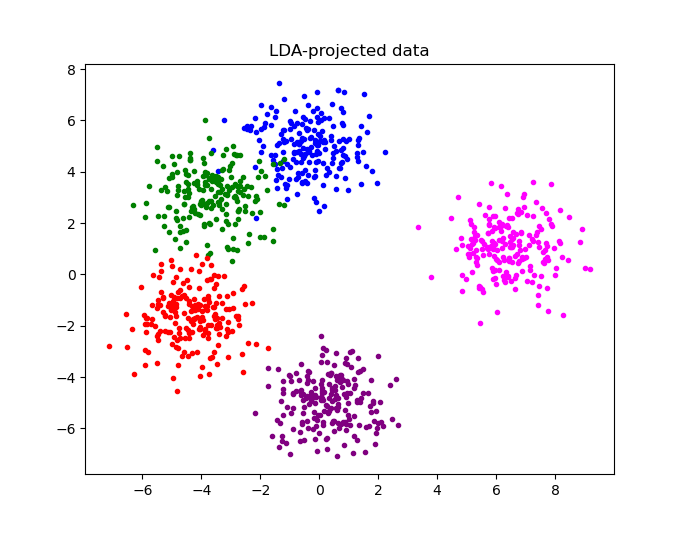
\includegraphics[width=\columnwidth]{figs/synthetic_projection.png}
    \caption{LDA projection of synthetic data in $\mathbb{R}^{100}$.}
    \label{fig:synthetic_projection}
\end{figure}

The results of this projection are shown in Figure \ref{fig:synthetic_projection}.
We find that LDA does indeed find a projection subspace that separates classes well, despite the subspace being very low-dimensional ($M=2$) when compared to the original feature space ($D=100$). 
This shows that when the assumptions of normality and homogeneity are satisfied, LDA is an effective tool to extract the most discriminating features from high-dimensional data.
In addition,
% to applying LDA to reduce the dimension of our synthetic data, we apply LDA to classify our synthetic data, and find that
because the classes were well separated and satisfied the assumptions of the model, LDA produced 100\% accuracy on the synthetic data when used as a classifier.

\subsection{LDA for Star Classification}
We use LDA to classify stars from a set of observable attributes.
More specifically, we classify stars as brown dwarfs, red dwarfs, white dwarfs, main sequence, supergiants, or hypergiants ($C=6$) depending on a number of their features present in our data~\cite{stardata}, namely the stars' temperature, radius, luminosity, absolute magnitude, apparent color, and spectral type ($D=6$).
% The exact conditions a star should meet to be considered one of these types is out of the scope of this project, but relevant to our experiment is the dependence of a star's type on a number of its features present in our data~\cite{stardata},
% Astronomers use these features to classify stars as one of the star types outlined above, so we use LDA to uncover the latent relationship.
Our data contains $N=240$ samples total, with each class containing $N_k=40$ observations.

We turn our attention to spectral type, which is an attribute of a star given by properties already present in our data, such as temperature and luminosity.
Critical to nearly all classification algorithms, LDA requires the data's attributes to be independent of each other, and in our testing, we find that excluding the spectral type results in a slightly more accurate model.

We train our model by randomly splitting our data into 70\% for training and 30\% for testing. 
% testing the accuracy of our model on the remaining 30\%.
% In one such split, our model achieved 98.61\% accuracy.
% However, to remove this score's dependence on the way in which we split the data, we ran the same process on 
Over 50 such splits, our model achieved a mean testing accuracy of 98.9\% with a standard deviation of 1.1\%.

\subsection{LDA for Data Visualization}
Though not discussed at great length in this paper, LDA can also be used as a tool to assist in the visualization of labeled data.
Due to limitations of human vision, visualization of data with dimensionality greater than 3 is unintuitive at best.
However, LDA's ability to optimally discriminate between classes during projection can provide an effective means to visualize the relationships between classes.
We briefly demonstrate this ability by projecting our star data to two dimensions and visualizing the results in Figure \ref{fig:starR2}.
\begin{figure}[h]
    \centering
    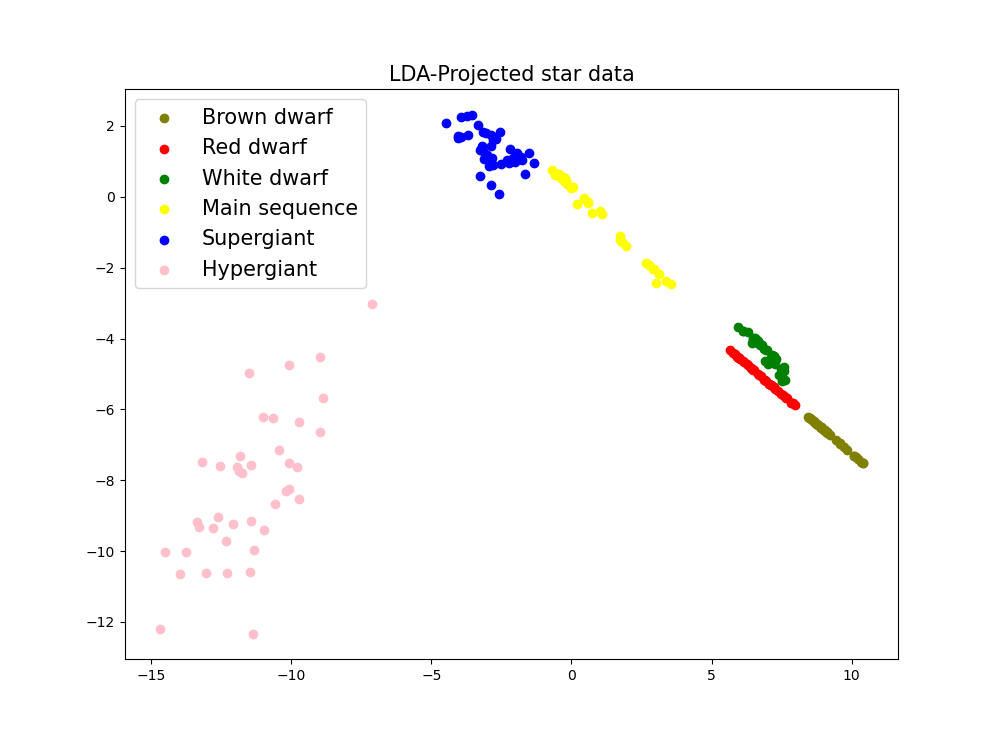
\includegraphics[width=\columnwidth]{figs/star_reduced.png}
    \caption{LDA reduction of star data to two dimensions.}
    \label{fig:starR2}
\end{figure}

Coincidentally, we find that LDA seems to approximate the structure of a Hertzsprung-Russell (HR) diagram, the standard diagram used to visualize star types in relation to their temperature and luminosity: see Figure \ref{fig:HRdiagram} for one such example.
\begin{figure}
    \centering
    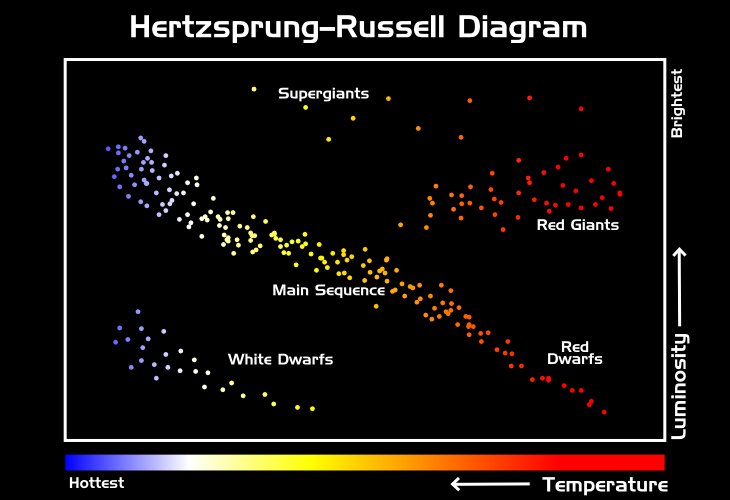
\includegraphics[width=\columnwidth]{figs/hrdiagram.png}
    \caption{Example of a Hertzsprung-Russell diagram.\\ Source: \url{http://aspire.cosmic-ray.org/Labs/StarLife/studying.html}}
    \label{fig:HRdiagram}
\end{figure}
The axes of the HR diagram are often simply temperature and luminosity, so we cannot expect the axes to be equivalent in our projection subspace, however the overall shape of the HR diagram is preserved modulo some affine transformation of our projected data points. 
There is a distinct diagonal main sequence branch, with white dwarfs clearly separated from the main sequence branch, and the giants diverging off to the opposite side of the white dwarfs.

%Note that the white dwarf class appears much closer in distance to the red dwarf class in our diagram than a typical HR diagram.
%We believe this is due to the presence of the star radius in our data as an attribute, and white dwarfs are similar to red dwarfs in radius.
%HR diagrams make no mention of radius on the axes, so the white dwarf class can be separated to a more arbitrary degree from the red dwarfs.
%Similarly, the hypergiant class stars appear more distant from our plot's main sequence branch, likely due for the same reason, where on the HR diagram, the lack of the star's radius being represented means giants can be placed closer to the main sequence branch.

\subsection{X-Ray Image Classification}
\citeauthor{lietal} \autocite{lietal} find that LDA is an effective multiclass classifier in facial and object recognition, despite the image data used in these tasks frequently violating the homogeneity assumption necessary for LDA.
In view of this, we want to explore LDA's robustness to highly variant data.

We consider the problem of diagnosing pneumonia in patients using images of their chest X-rays. Our training dataset consists of a set of $N=2250$ grayscale chest X-ray images with varying dimensions belonging to $C=3$ classes (with $N_k=750$ for each class) that have been sampled from a database of around 5000 images \autocite{kermanyetal2018}. In order to standardize the dimensionality of the dataset, we resize all images to dimensions $220\times 220$ pixels and flatten each image array to generate our dataset $\{\ve{x}_i\}_{i=1}^{2250} \subset \mathbb{R}^{220*220}$. Then, we apply horizontal and vertical Sobel filters to each image in order to exploit some common differences between normal and pneumonia X-rays, such as some cloudiness in the ribcage as seen in the pneumonia X-rays in Figure \ref{fig:xrays}.

Each image is classified with one of three diagnoses: normal, bacterial pneumonia, or viral pneumonia. Our classification technique takes two steps: We first consider all three diagnosis types as separate classes in order to reduce the dimension of each $\ve{x}_i$ to 2 using the LDA technique described in section \ref{subsec:dimreduct}. Then, in order to optimally train our binary classifier, we group both types of pneumonia under a single class and sample 750 images from this new class to maintain evenness between the size of our classes. Finally, we apply a binary classifier to the dimensionality-reduced data. 
\begin{figure}
    \centering
    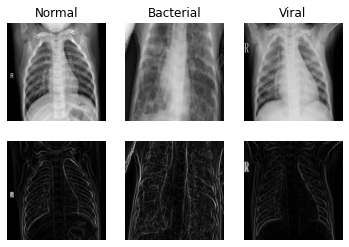
\includegraphics[width=\columnwidth]{figs/X-rays.png}
    \caption{X-ray images with and without Sobel filter.}
    \label{fig:xrays}
\end{figure}
\begin{figure}
    \centering
    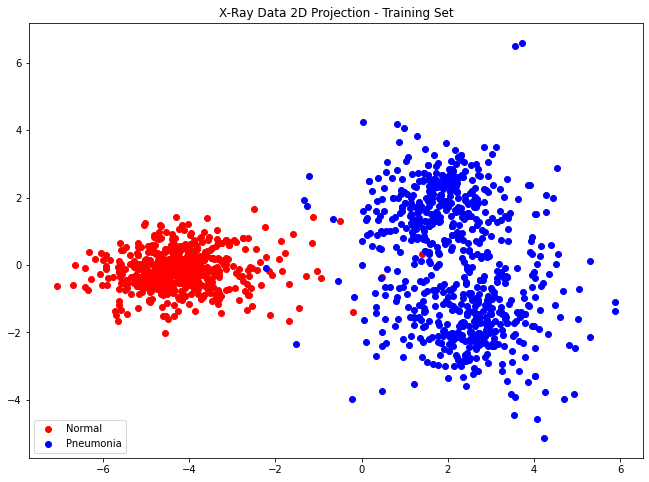
\includegraphics[width=\columnwidth]{figs/X-ray proj.png}
    \caption{Projection of training set to two dimensions.}
    \label{fig:xrayproj}
\end{figure}
\begin{figure}
    \centering
    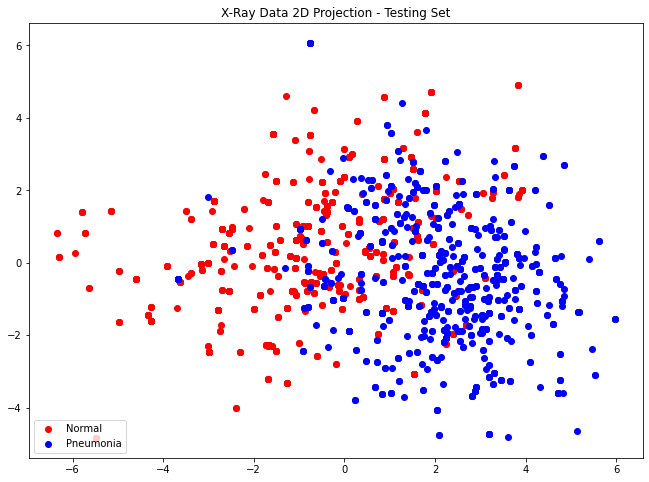
\includegraphics[width=\columnwidth]{figs/X-rayprojtest.png}
    \caption{Projection of test set to two dimensions using model from training set.}
    \label{fig:xrayprojtest}
\end{figure}
Figure \ref{fig:xrays} shows a sample of images from the dataset. After finding the two eigenvectors satisfying Fisher's criterion for the training dataset, we plot the projection of the data onto the subspace spanned by this basis, which is shown in Figure \ref{fig:xrayproj}. The projection of the test dataset using the train-fitted subspace is shown in Figure \ref{fig:xrayprojtest}. The training dataset seems to be well separated due to overfitting of the LDA model to the training set. Nevertheless, our various binary classifiers, such as logistic regression, SVM, and binary LDA all achieve a prediction accuracy rate of about 70\% without a Sobel filter and 75\% with a Sobel filter.

In addition to overfitting of the model, we can also explain the poor generalization of the train-fitted projection subspace to the test data by noting the high variance of our data.
Figure \ref{fig:xrays} shows the variation in anatomy and positioning, causing the images to be highly irregular.
To improve LDA's performance on this dataset, one should consider restricting the dataset to images that are controlled for body type, positioning, etc. or consider another regularization routine to reduce the variance of the data.


\section{Advantages and Disadvantages}\label{sec:Advantages and Disadvantages}
One of LDA's most useful features is its ability to reduce the dimensionality of data while also serving as a robust classifier method. This enables us to visualize data in lower dimensions, allowing for easily interpretable results. 
The fact that the decision boundary is linear means that the algorithm is easy to implement and yields a simple but robust classification model.

One of LDA's disadvantages is that it is perhaps too simple. A linear decision boundary may not yield an adequate classification accuracy. The assumption of normally distributed data also limits its ability to work with more complex datasets. In the high dimensional problem, if the sample size is small, it becomes impossible to solve for eigenvalues and eigenvectors of $\ve{S}_w^{-1}\ve{S}_b$ without modifications to the derivation.

Our experiment with the chest X-ray dataset also points to LDA showing a lack of robustness to highly variable data, with its ability to discriminate classes not generalizing well to test data when the train data is highly variable with many attributes.

\section{CONCLUSIONS}\label{sec:conclusions}
In this paper, we explained the mathematical foundations of LDA and applied it to various types of classification and dimension reduction problems in order to demonstrate its efficacy. We have used Fisher's criterion to solve for the optimal directions of projection and considered the application of Bayes' theorem to the general multiclass classification problem.

In our experiments, we have applied LDA to a synthetic data set in order to showcase its performance in the multiclass classification problem, yielding promising results despite the reduction of a 100-dimensional space to a 2-dimensional space. We achieved a high degree of accuracy when applying LDA for star classification while demonstrating LDA's data visualization capabilities by comparing its results to the Hertzsprung-Russell diagram. Finally, we obtained surprisingly accurate results when using LDA to help diagnose instances of pneumonia in a highly variant dataset of X-ray images.
All content of this project, including the code for our experiments, are available on our GitHub repository: \url{https://github.com/warewaware/LDA156FinalProj}.
\printbibliography


\addtolength{\textheight}{-12cm}   % This command serves to balance the column lengths
                                  % on the last page of the document manually. It shortens
                                  % the textheight of the last page by a suitable amount.
                                  % This command does not take effect until the next page
                                  % so it should come on the page before the last. Make
                                  % sure that you do not shorten the textheight too much.

%%%%%%%%%%%%%%%%%%%%%%%%%%%%%%%%%%%%%%%%%%%%%%%%%%%%%%%%%%%%%%%%%%%%%%%%%%%%%%%%



%%%%%%%%%%%%%%%%%%%%%%%%%%%%%%%%%%%%%%%%%%%%%%%%%%%%%%%%%%%%%%%%%%%%%%%%%%%%%%%%



%%%%%%%%%%%%%%%%%%%%%%%%%%%%%%%%%%%%%%%%%%%%%%%%%%%%%%%%%%%%%%%%%%%%%%%%%%%%%%%%
%\section*{APPENDIX}



%\section*{ACKNOWLEDGMENT}





%%%%%%%%%%%%%%%%%%%%%%%%%%%%%%%%%%%%%%%%%%%%%%%%%%%%%%%%%%%%%%%%%%%%%%%%%%%%%%%%






\end{document}
